\begin{frame}[plain, c]
    \centering
    \vspace{5em}
    \Huge
    Agentic AI
\end{frame}


\begin{frame}{}
  \centering
  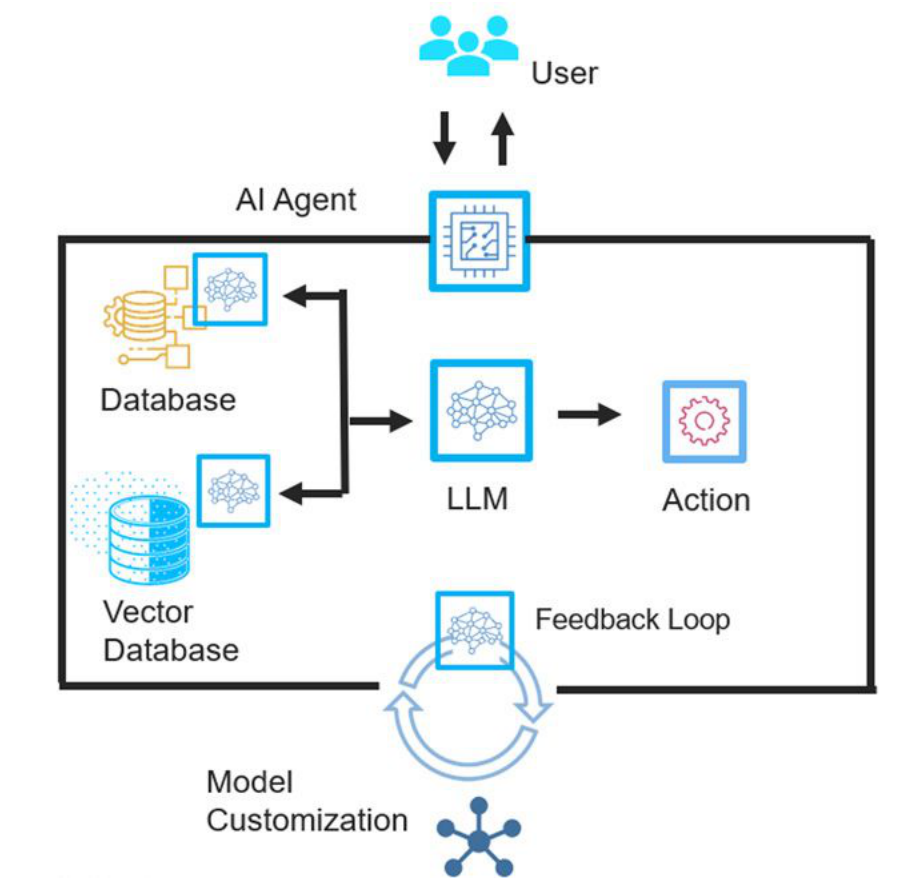
\includegraphics[width=0.98\textwidth, height=0.98\textheight, keepaspectratio]{assets/Lecture-10_Multimodal_NLP_Agentic_AI/slide_030.png}
\end{frame}

\begin{frame}{What is Agentic AI?}
  \begin{itemize}
    \item[\textcolor{red}{$\triangleright$}] AI systems that \textbf{perceive, reason, plan,} and \textbf{act} to fulfill goals.
    \item[\textcolor{red}{$\triangleright$}] \textbf{Agent loop:} Observe $\rightarrow$ Plan $\rightarrow$ Act $\rightarrow$ Reflect $\rightarrow$ Learn
    \item[\textcolor{red}{$\triangleright$}] Inspired by cognitive science, robotics, and autonomous agents.
  \end{itemize}
  \vspace{1em}
  \textbf{Core Components:}
  \begin{itemize}
    \item[\textcolor{red}{$\triangleright$}] Memory
    \item[\textcolor{red}{$\triangleright$}] Planning
    \item[\textcolor{red}{$\triangleright$}] Tool-use (plugins, APIs)
    \item[\textcolor{red}{$\triangleright$}] Feedback-driven behavior
  \end{itemize}
\end{frame}

\begin{frame}{What is Agentic AI?}
  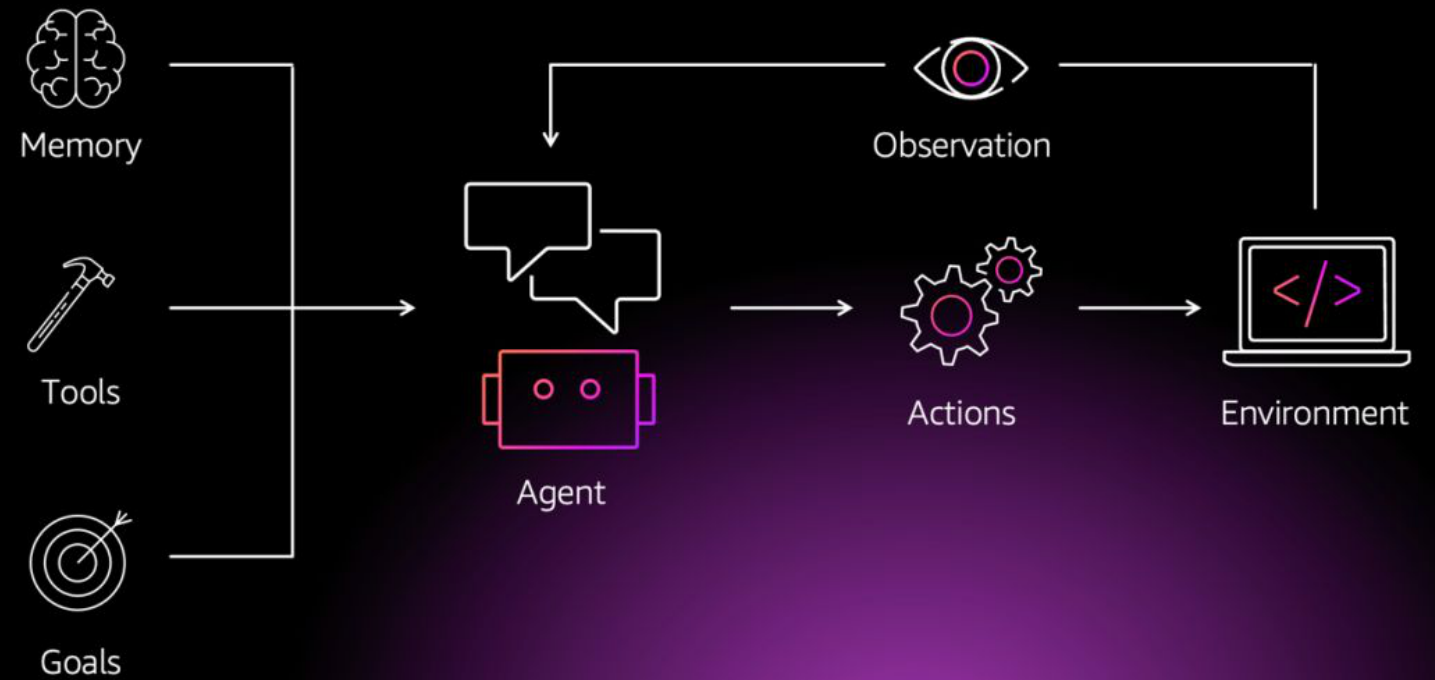
\includegraphics[width=0.98\textwidth, height=0.98\textheight, keepaspectratio]{assets/Lecture-10_Multimodal_NLP_Agentic_AI/slide_032.png}
\end{frame}

\begin{frame}{Reactive vs. Proactive Agents}
  \begin{table}[h!]
    \centering
    \begin{tabular}{l l l}
      \textbf{Feature} & \textbf{Reactive} & \textbf{Proactive} \\
      \hline
      Response & Immediate & Goal-oriented \\
      Planning & None & Yes \\
      Learning & Event-triggered & Self-initiated \\
      Example & Chatbots & Auto-GPT, Personal Assistants \\
    \end{tabular}
  \end{table}
  \vspace{1em}
  \textbf{Proactive agents} generate goals, schedule actions, and evaluate results even without user prompts.
\end{frame}

\begin{frame}{Reactive vs. Proactive Agents}
    \centering
    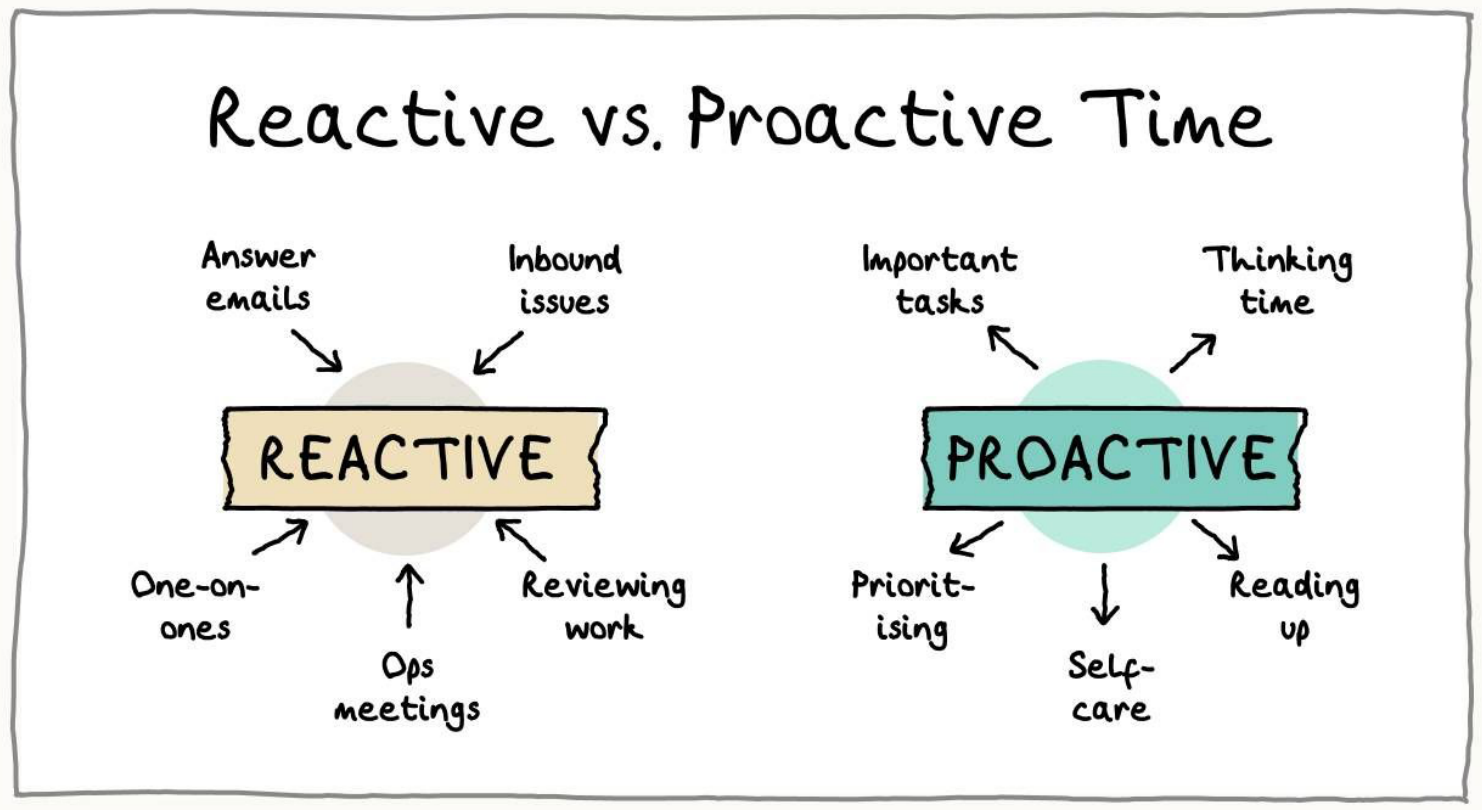
\includegraphics[width=0.98\textwidth, height=0.98\textheight, keepaspectratio]{assets/Lecture-10_Multimodal_NLP_Agentic_AI/slide_034.png}
\end{frame}

\begin{frame}{Reactive vs. Deliberative Agents}
  \centering
  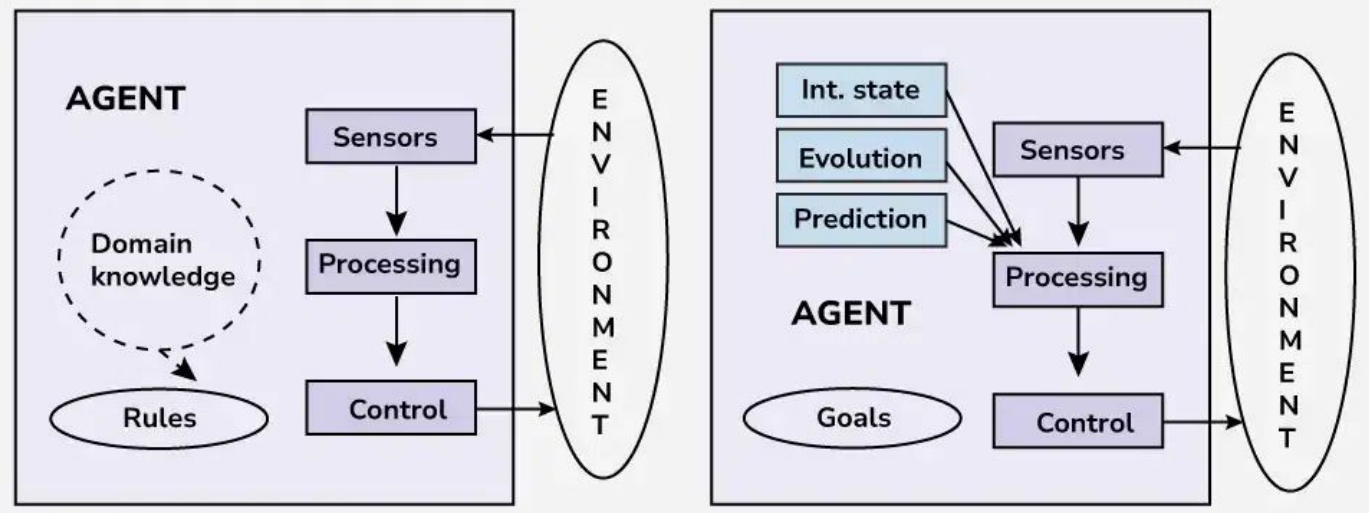
\includegraphics[width=0.98\textwidth, height=0.98\textheight, keepaspectratio]{assets/Lecture-10_Multimodal_NLP_Agentic_AI/slide_035.png}
\end{frame}

\begin{frame}{Reactive vs. Proactive Agents}
  \centering
  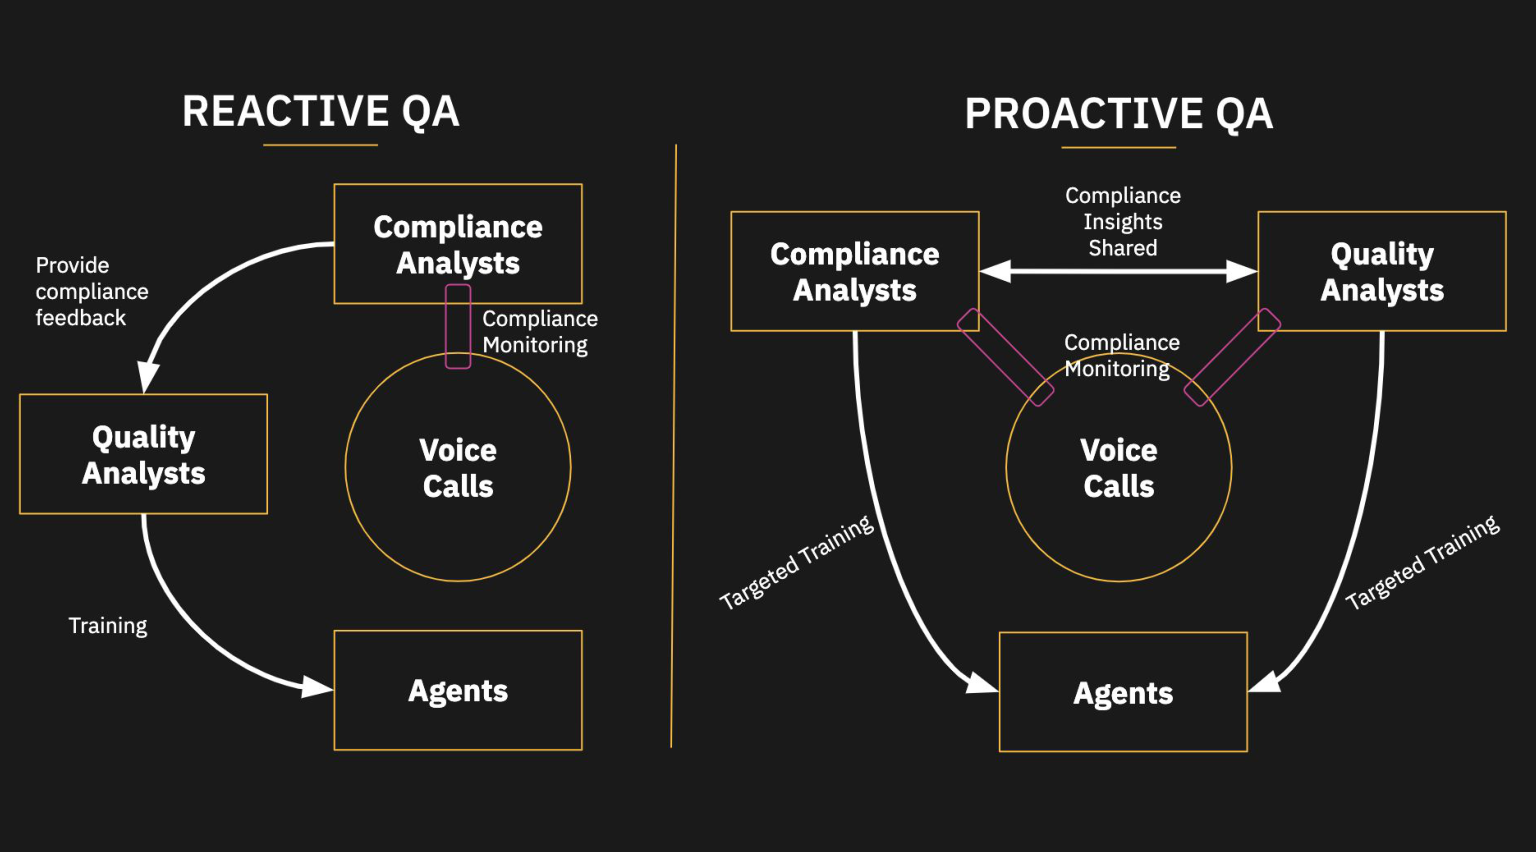
\includegraphics[width=0.98\textwidth, height=0.98\textheight, keepaspectratio]{assets/Lecture-10_Multimodal_NLP_Agentic_AI/slide_036.png}
\end{frame}

\begin{frame}{Agent Loop in Detail}
  \textbf{\textcolor{red}{\large $\triangleright$ Perceive:}}~Multimodal input (text, vision, memory) \\
  \textbf{\textcolor{red}{\large $\triangleright$ Interpret:}}~NLP/vision models \\
  \textbf{\textcolor{red}{\large $\triangleright$ Plan:}}~Task decomposition (e.g., LangChain chains) \\
  \textbf{\textcolor{red}{\large $\triangleright$ Act:}}~API/tool calling \\
  \textbf{\textcolor{red}{\large $\triangleright$ Reflect \& Learn:}}~Refine memory or adjust goals
  \vspace{1em}
  
  \textbf{Applications:}
  \begin{itemize}
    \item[\textcolor{red}{$\triangleright$}] Personal AI assistants
    \item[\textcolor{red}{$\triangleright$}] Research co-pilots
    \item[\textcolor{red}{$\triangleright$}] Automated workflows
  \end{itemize}
\end{frame}

\begin{frame}{Agentic RAG Workflow}
  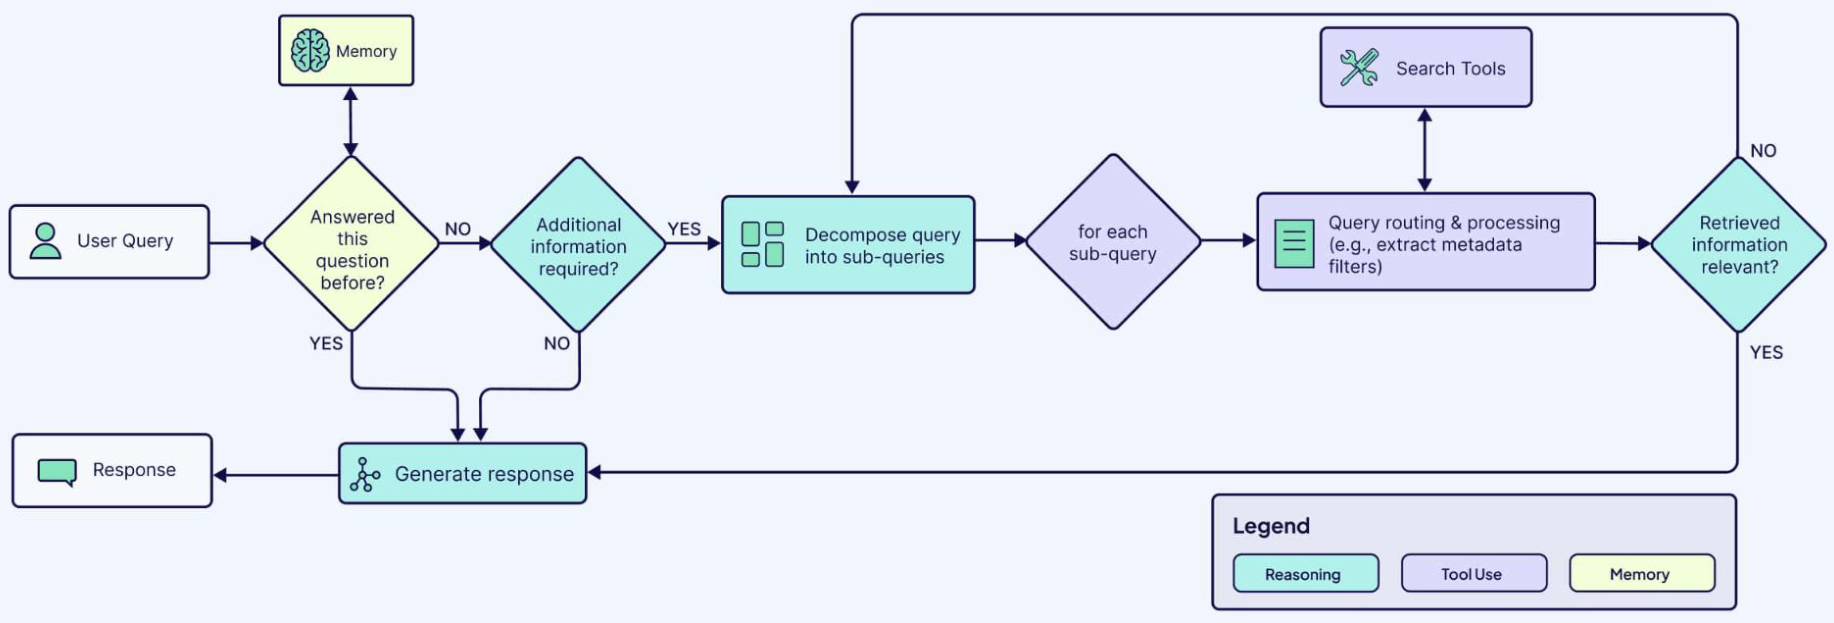
\includegraphics[width=0.98\textwidth, height=0.98\textheight, keepaspectratio]{assets/Lecture-10_Multimodal_NLP_Agentic_AI/slide_038.png}
\end{frame}

\begin{frame}{Open-Source Agentic Frameworks}
  \centering
  \Huge Open-Source Agentic Frameworks
\end{frame}

\begin{frame}{Auto-GPT}
  \centering
  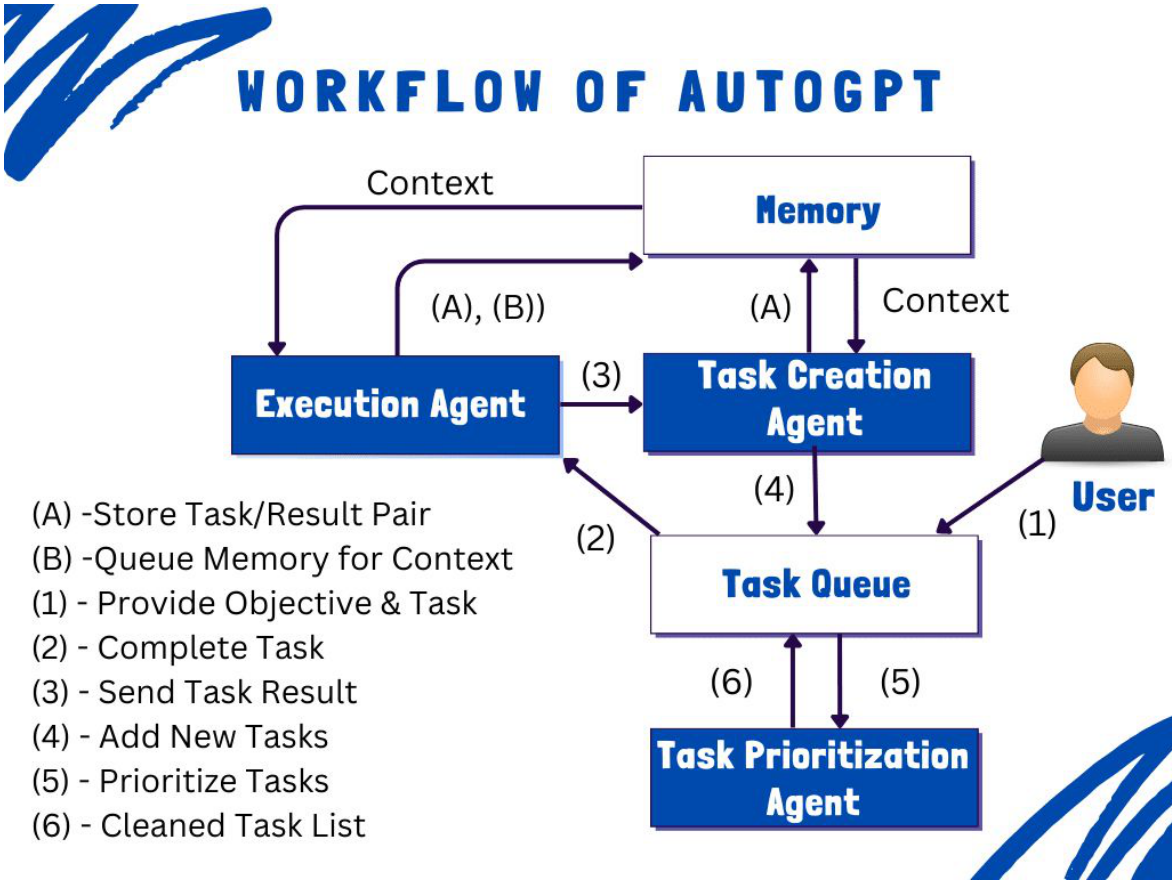
\includegraphics[width=0.98\textwidth, height=0.98\textheight, keepaspectratio]{assets/Lecture-10_Multimodal_NLP_Agentic_AI/slide_040.png}
\end{frame}

\begin{frame}{Auto-GPT}
    \textbf{Auto-GPT} is an \textbf{open-source project} that chains GPT calls to build autonomous agents.
    \begin{itemize}
        \item[\textcolor{red}{$\triangleright$}] \textbf{Open-source project} that chains GPT calls to build autonomous agents.
        \item[\textcolor{red}{$\triangleright$}] Uses \textbf{long-term memory}, file storage, and self-generated tasks.
        \item[\textcolor{red}{$\triangleright$}] \textbf{Requirements:}
        \begin{itemize}
            \item Task input
            \item Internet / API access
            \item Feedback loop
        \end{itemize}
    \end{itemize}
    \vspace{0.5em}
    \textbf{GitHub:} \href{https://github.com/Torantulino/Auto-GPT}{https://github.com/Torantulino/Auto-GPT}
\end{frame}

\begin{frame}{Auto-GPT}
  \centering
  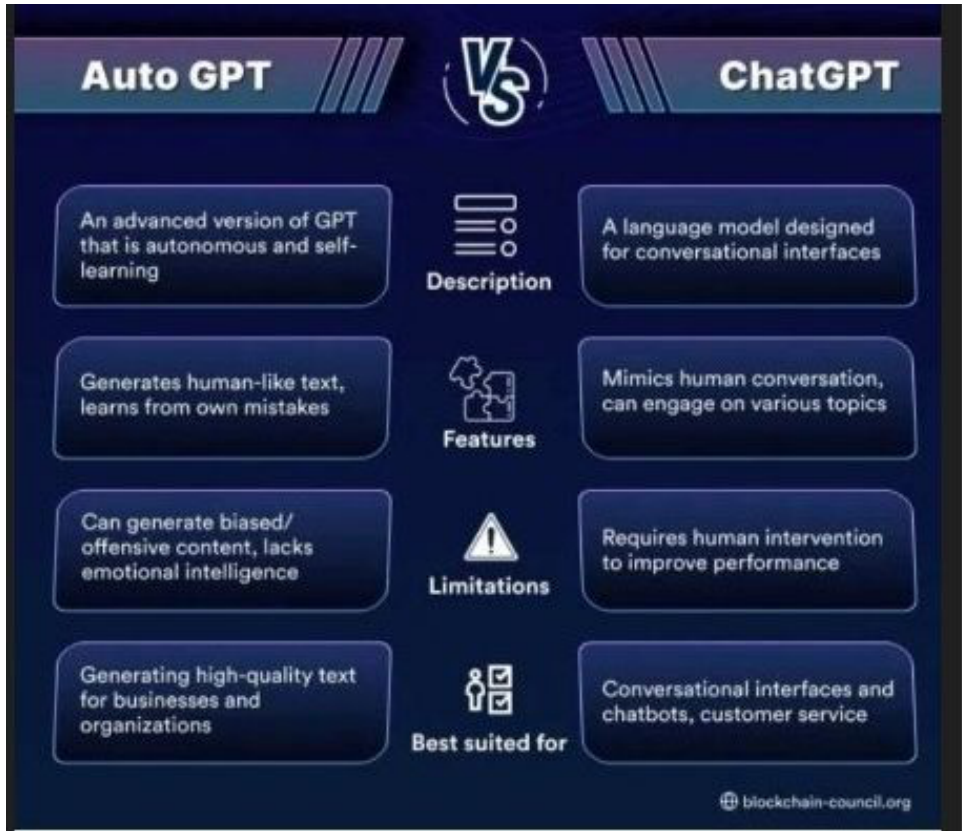
\includegraphics[width=0.98\textwidth, height=0.98\textheight, keepaspectratio]{assets/Lecture-10_Multimodal_NLP_Agentic_AI/slide_042.png}
\end{frame}

\begin{frame}{BabyAGI}
  \centering
  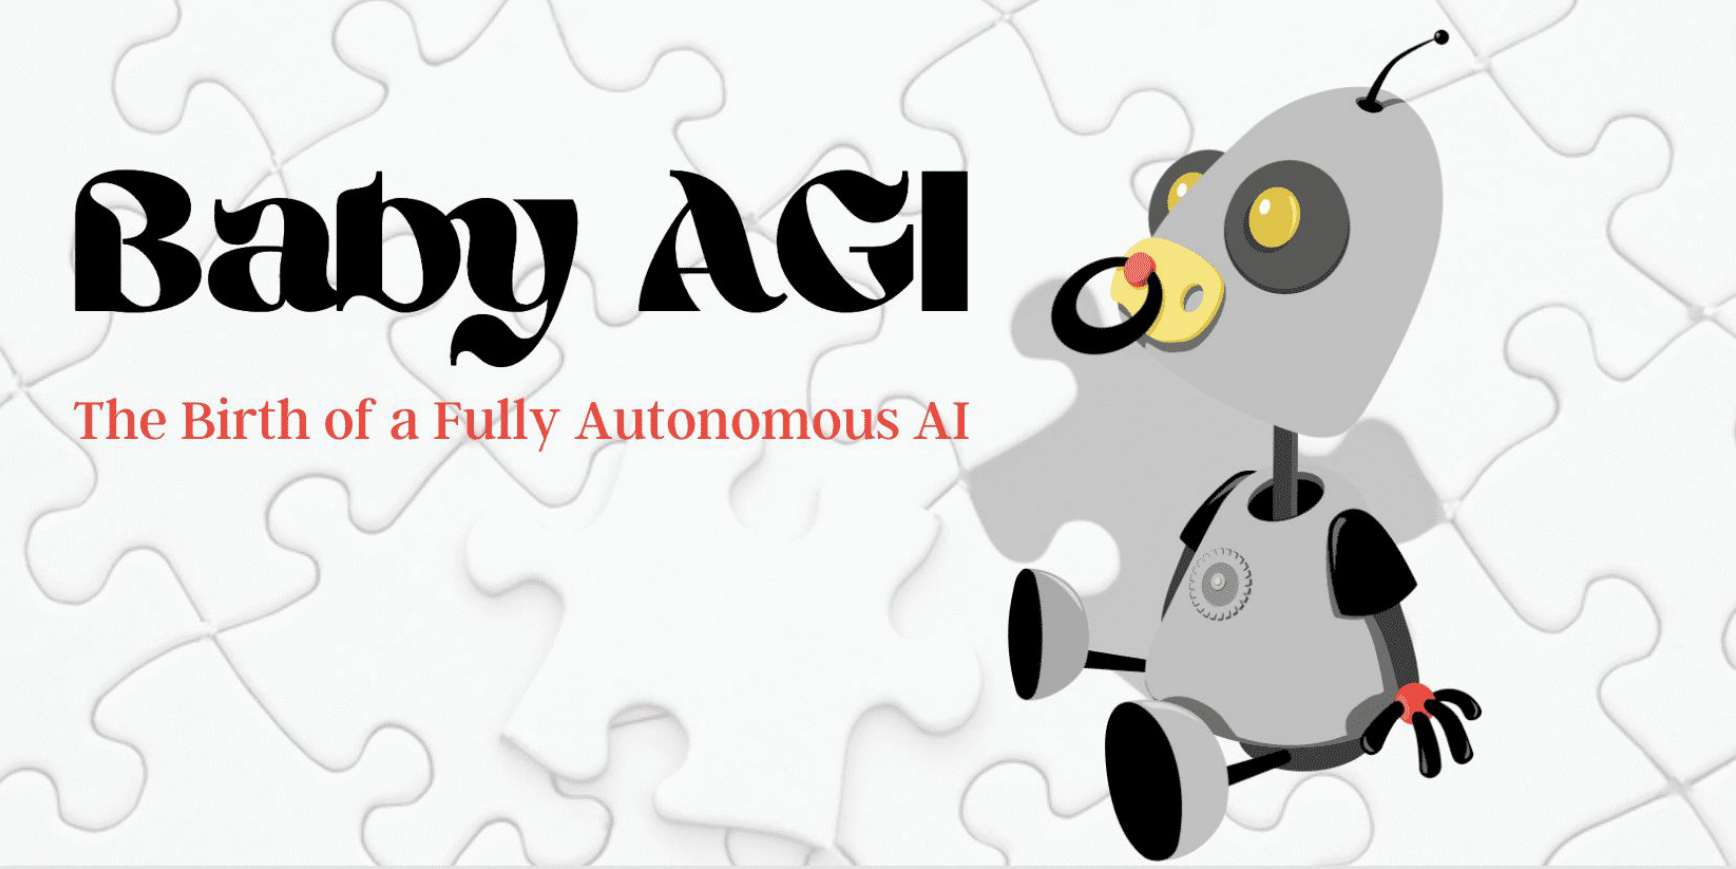
\includegraphics[width=0.98\textwidth, height=0.98\textheight, keepaspectratio]{assets/Lecture-10_Multimodal_NLP_Agentic_AI/slide_043.png}
\end{frame}

\begin{frame}{BabyAGI}
    \begin{itemize}
        \item[\textcolor{red}{$\triangleright$}] \textbf{Lightweight Python agent loop}
        \item[\textcolor{red}{$\triangleright$}] Generates tasks from high-level objectives
        \item[\textcolor{red}{$\triangleright$}] Runs tasks, stores results, and generates new tasks iteratively
        \item[\textcolor{red}{$\triangleright$}] Emphasizes simplicity and minimalism
    \end{itemize}
    \vspace{0.5em}
    \textbf{GitHub:} \href{https://github.com/yoheinakajima/babyagi}{https://github.com/yoheinakajima/babyagi}
\end{frame}


\begin{frame}{BabyAGI: How BabyAGI Works}
  \centering
  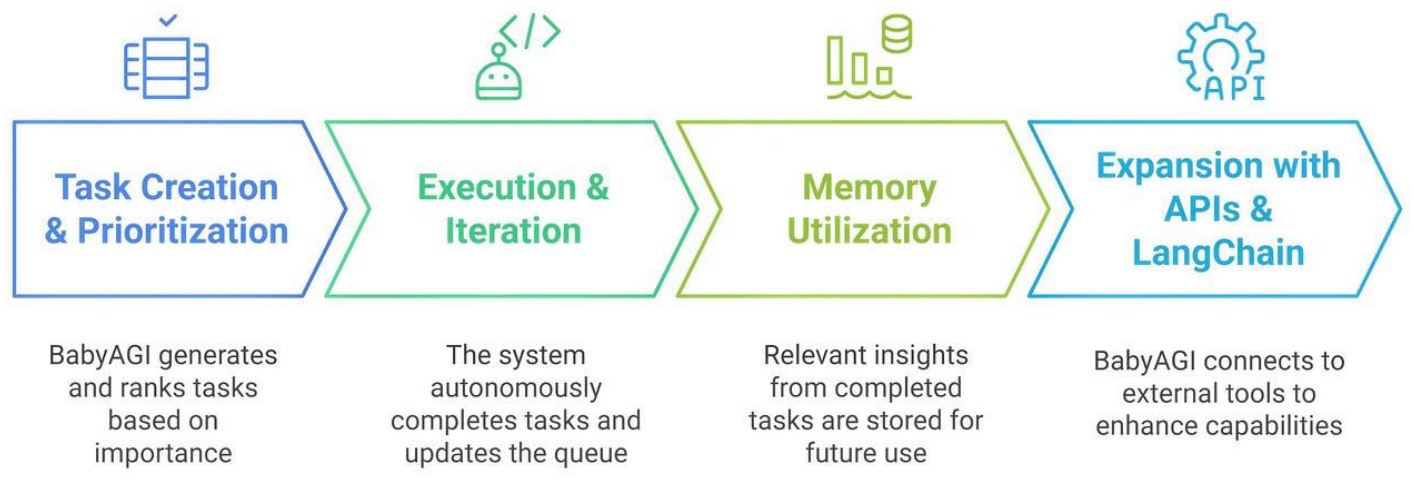
\includegraphics[width=0.98\textwidth, height=0.98\textheight, keepaspectratio]{assets/Lecture-10_Multimodal_NLP_Agentic_AI/slide_046.png}
\end{frame}

\begin{frame}{Other Notable Frameworks}
  \begin{itemize}
    \item[\textcolor{red}{$\triangleright$}] \textbf{LangChain:} Framework for chaining LLMs with tools, APIs, and memory. Enables complex workflows and agentic behavior.
    \item[\textcolor{red}{$\triangleright$}] \textbf{CrewAI:} Multi-agent coordination platform for collaborative task execution.
    \item[\textcolor{red}{$\triangleright$}] \textbf{SuperAGI:} Production-grade agent platform supporting extensibility, monitoring, and deployment.
    \item[\textcolor{red}{$\triangleright$}] \textbf{OpenDevin:} Developer-oriented agentic IDE for automating software engineering tasks.
  \end{itemize}
\end{frame}

\begin{frame}{LangChain}
  \centering
  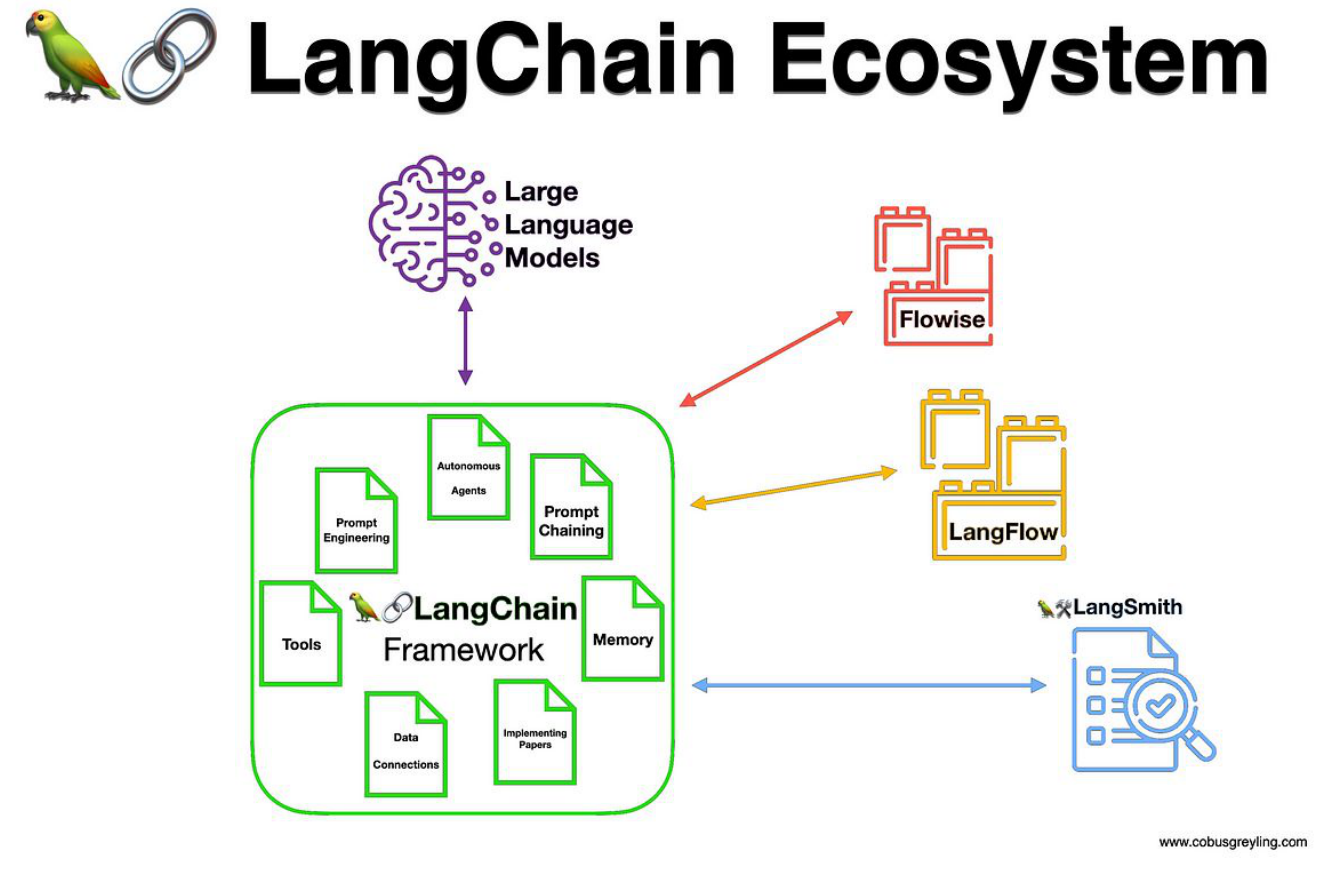
\includegraphics[width=0.98\textwidth, height=0.98\textheight, keepaspectratio]{assets/Lecture-10_Multimodal_NLP_Agentic_AI/slide_048.png}
\end{frame}

\begin{frame}{CrewAI}
  \centering
  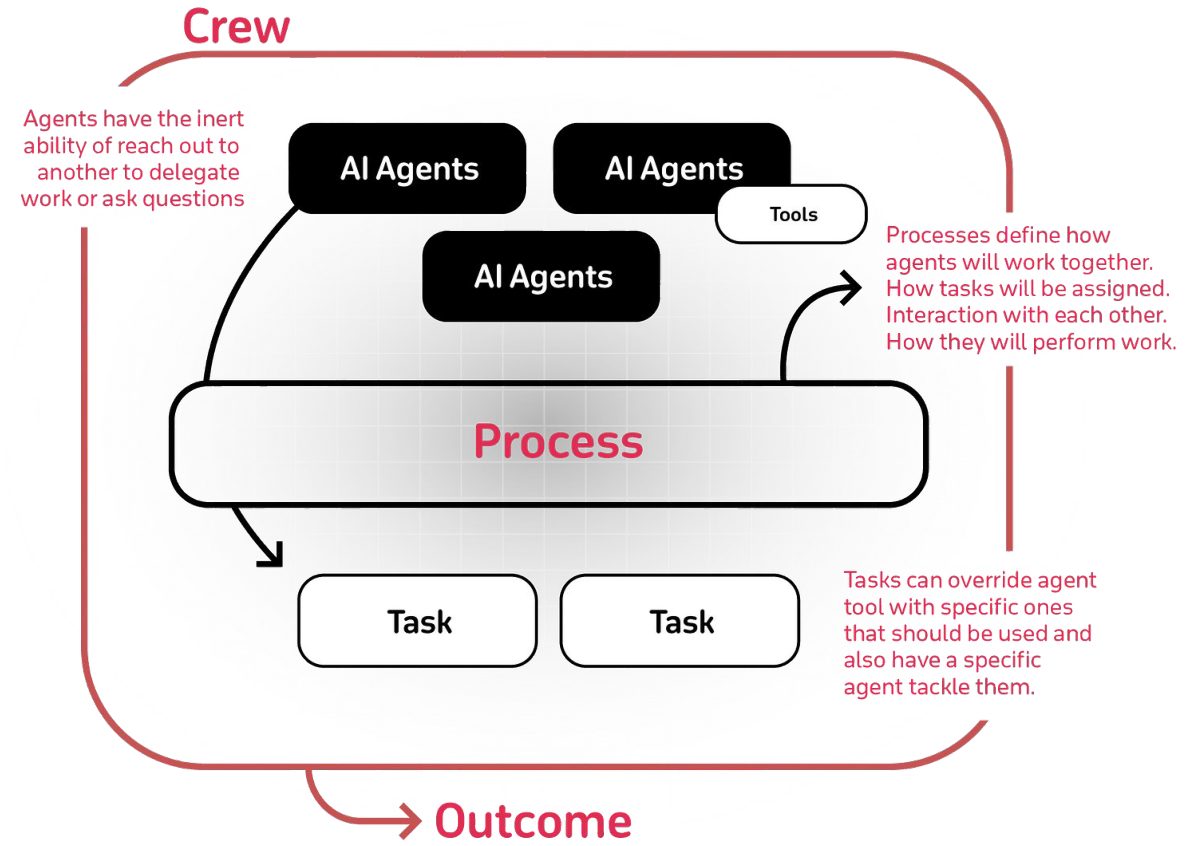
\includegraphics[width=0.98\textwidth, height=0.98\textheight, keepaspectratio]{assets/Lecture-10_Multimodal_NLP_Agentic_AI/slide_049.png}
\end{frame}

\begin{frame}{SuperAGI}
  \centering
  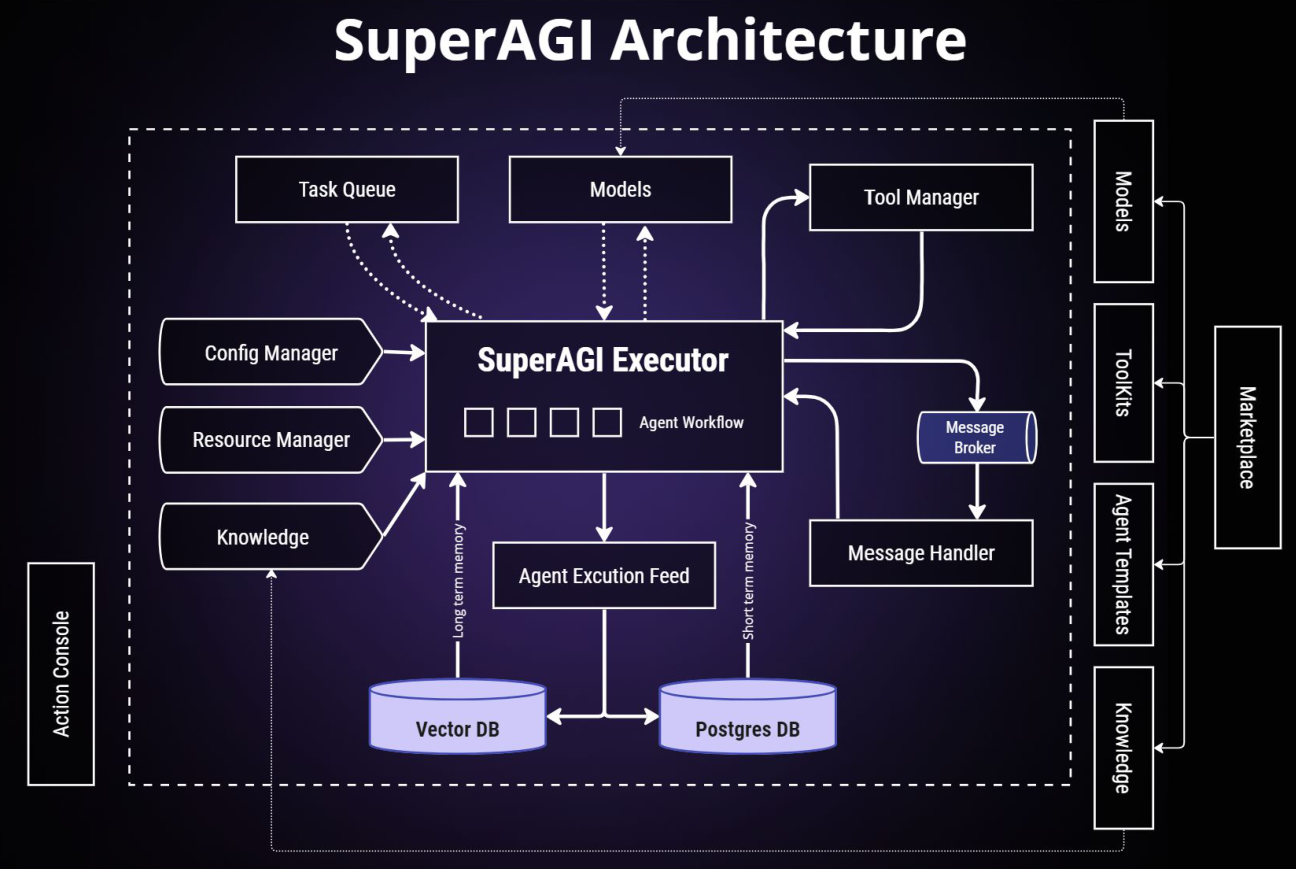
\includegraphics[width=0.98\textwidth, height=0.98\textheight, keepaspectratio]{assets/Lecture-10_Multimodal_NLP_Agentic_AI/slide_050.png}
\end{frame}

\begin{frame}{SuperAGI}
  \centering
  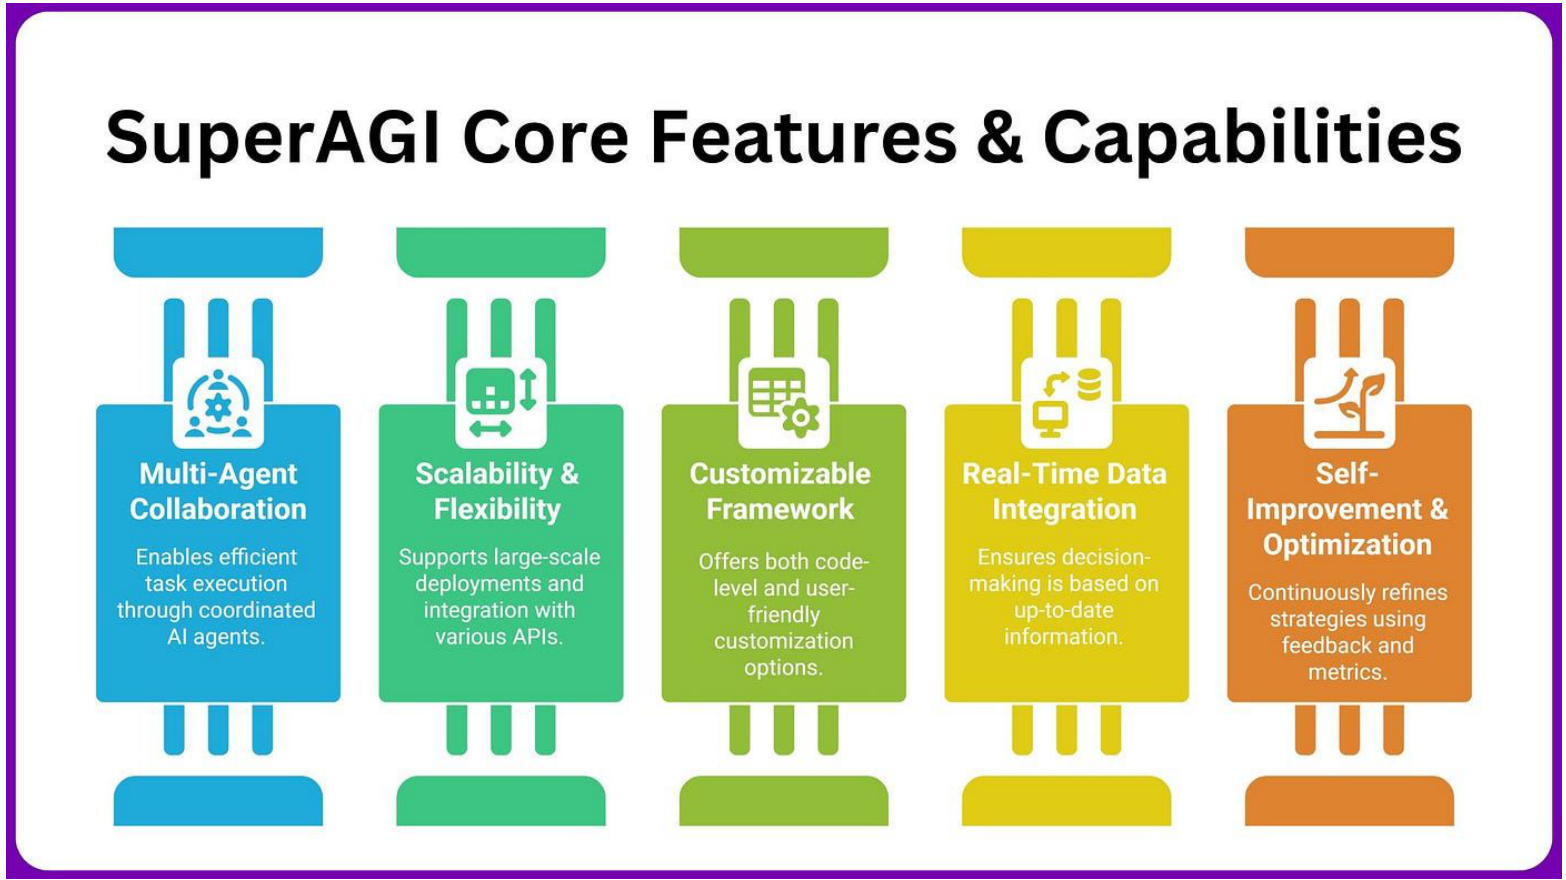
\includegraphics[width=0.98\textwidth, height=0.98\textheight, keepaspectratio]{assets/Lecture-10_Multimodal_NLP_Agentic_AI/slide_051.png}
\end{frame}

\begin{frame}{OpenDevin}
  \centering
  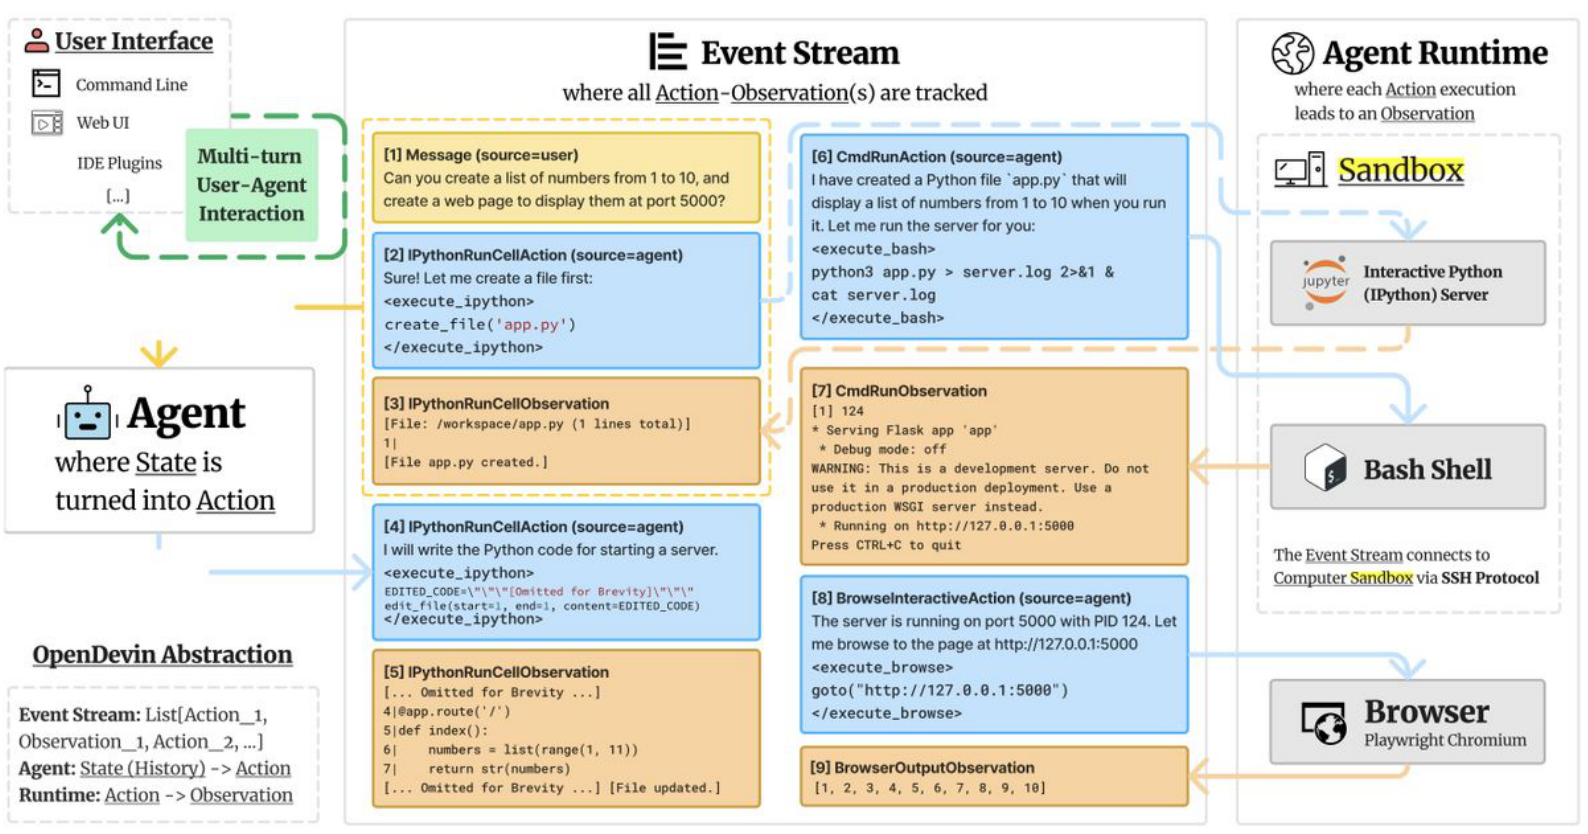
\includegraphics[width=0.98\textwidth, height=0.98\textheight, keepaspectratio]{assets/Lecture-10_Multimodal_NLP_Agentic_AI/slide_052.png}
\end{frame}
